\headline{{\textbf{\Large\sffamily Wired for Bonsai}}\\
          {\textbf{\large\sffamily YouTube Creators Off\--Camera \& Unfiltered}}}
\label{2025-11-wired}
\noindent
This month we have the pleasure of welcoming a special guest who truly needs no introduction. 
With more than 210\,000 followers and close to 2\,000 videos published over twelve years, \textbf{Nigel Saunders} has become one of the most recognisable and beloved figures in the online bonsai world. 
His channel, \textit{The Bonsai Zone}, is followed by beginners, professionals, and curious passers\--by alike, drawn in by his naturalistic approach, quiet determination, and willingness to show not only the triumphs, but also the setbacks that come with a life lived among miniature trees.

Nigel is known for his humility, his steady experimentation, and his unique ability to welcome viewers---expert or novice---straight into the heart of his greenhouse. 
In his videos he documents daily bonsai work alongside side projects as imaginative as his trees. 
Today, though, we try to step a little outside the greenhouse; to learn how it all began, and how Nigel's approach evolved into what millions enjoy today.

\medskip
\topic{Life Before Bonsai}
\noindent
When we ask Nigel where his journey began, he smiles and starts at the very beginning: ``\textit{I'm Nigel Saunders, and I live in South Western Ontario, Canada---about an hour and a half from Toronto.}'' 

Long before bonsai, long before YouTube, Nigel spent most of his professional life as a product designer, later transitioning into 3D design and rendering for stage productions. 
It was a career rooted firmly in the arts, and one that aligned naturally with the creative instincts that would later shape his bonsai practice. 
``\textit{I\hfill was\hfill always\hfill strong\hfill in\hfill the\hfill arts\hfill and\hfill took\hfill a}

\begin{window}[2,l,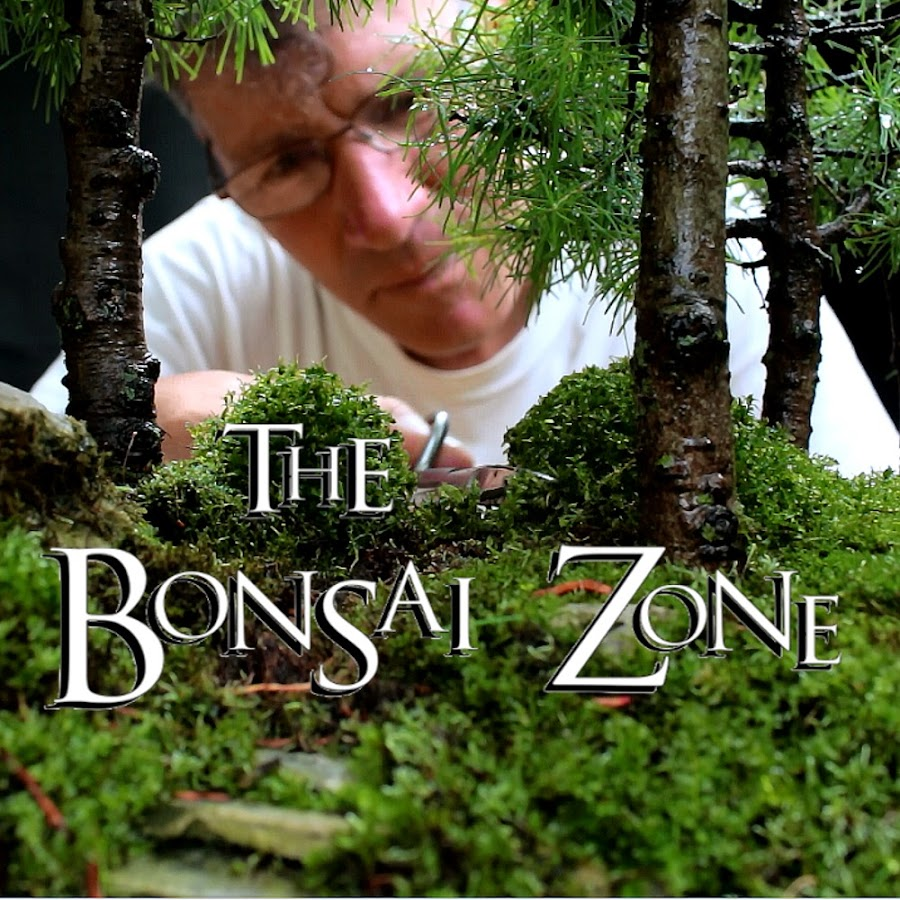
\includegraphics[width=1.0\columnwidth]{2025_11/res/wired_nigel},\centerline{\emph{Nigel Saunders towering over his magnificent creation:}}\\\centerline{\emph{A 'Giant' in the YouTube Bonsai World.}}]
\end{window}
\columnbreak

\noindent
\textit{creative approach to my work},'' he says, noting how design, composition, and visual problem\--solving became second nature.

His artistic inclinations stretch back even further---into childhood, where miniature worlds already played a prominent role.
``\textit{I was always into making models and miniatures for the Super~8 movies I made when I was young.}''
Drawing, painting, sculpting, model\--making: each contributed to an ever\--deepening fascination with recreating the world in small scale.
Bonsai, though he didn't yet know it, would become the ultimate expression of that impulse.

Nature, too, had always been a quiet background presence.
Nigel enjoyed trees and landscapes, but it wasn't until his introduction to bonsai that this early appreciation blossomed into a lifelong passion.
He credits not only books and magazines, but also fellow club members and the internet---with shaping the way he approaches creativity.
Rather than studying other artists' bonsai, he prefers observing trees in nature.
``\textit{Bonsai is my attempt and interpretation of the world around me.}''

\medskip
\topic{Learning Bonsai}
\noindent
Nigel's bonsai story begins, somewhat improbably, with an office Christmas gift.
At work, employees were given poinsettias to place on their desks.
In the soil of Nigel's plant, a tiny seedling had sprouted.
It turned out to be a \textit{Ficus microcarpa}.
As it grew, he eventually needed to prune it---and in searching the bookstore for a pruning guide, he found instead a book on bonsai.

``\textit{I was shocked that pruning trees was a hobby!}'' he laughs.
The discovery was instant and lasting: ``\textit{When I saw that first bonsai book, I was hooked for life.}''

Remarkably, Nigel still has that very same tree.
It continues to grow and evolve more than three decades later---a living record of his entire bonsai journey.

His early fascinations revolved around tropical rainforest species, especially those with strong aerial and buttressed roots.\hfill
Ficus\hfill and\hfill Schefflera\hfill remain\hfill favourites,\hfill though\hfill Nigel\hfill is

\begin{window}[2,l,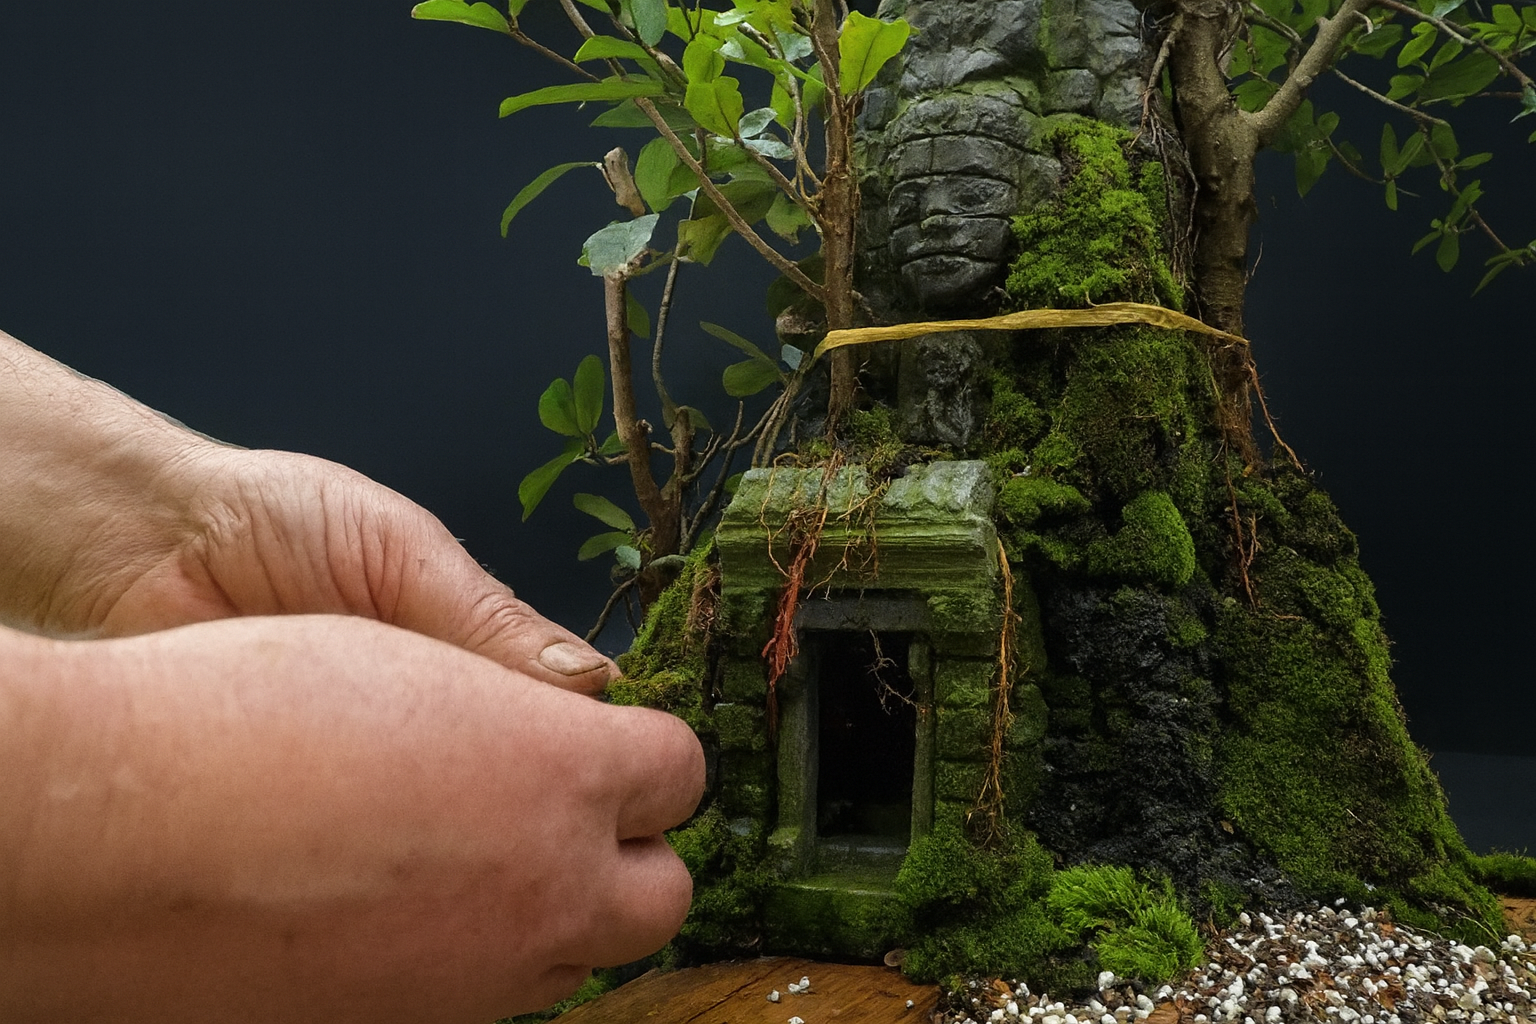
\includegraphics[width=1.0\columnwidth]{2025_11/res/wired_ta_prohm_temple},\centerline{\emph{Hand\--cast cement details and ficus trees}}\\\centerline{\emph{elevate Nigel's famous Ta Prohm temple penjing.}}]
\end{window}
\pagebreak
\vspace*{-3em}
\begin{window}[2,l,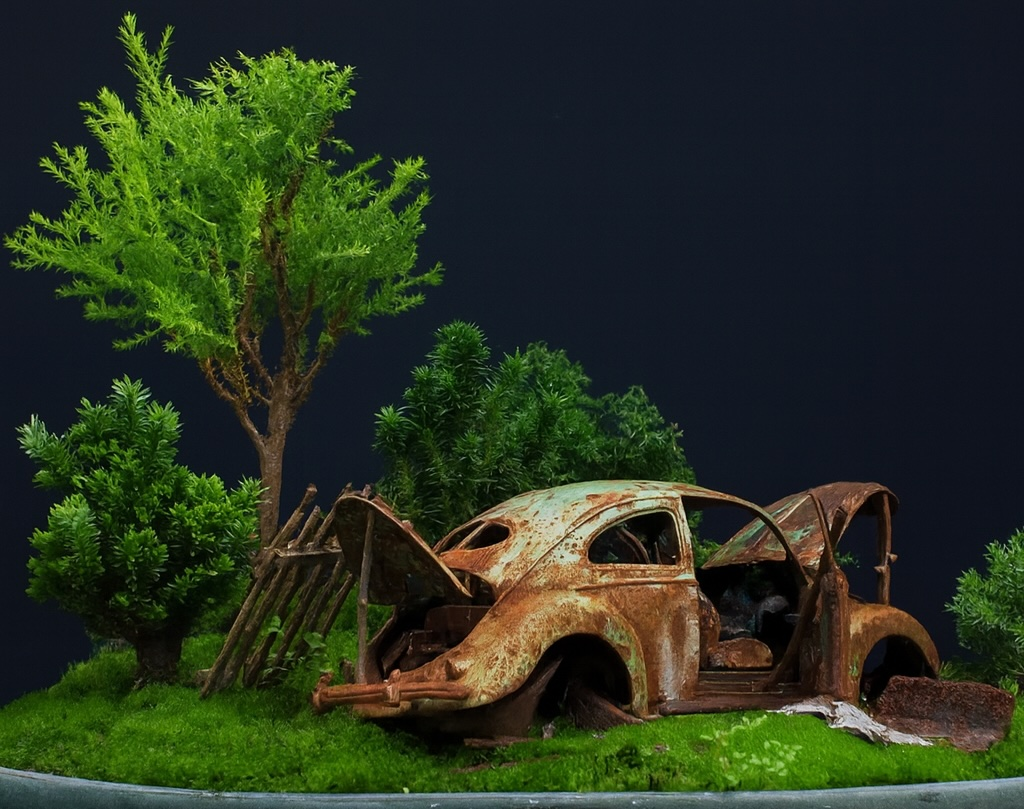
\includegraphics[width=1.0\columnwidth]{2025_11/res/wired_abandoned_beetle},\centerline{\emph{The iconic 'Abandoned Beetle' penjing highlights}}\\\centerline{\emph{Nigel's diverse modelling and miniature skills.}}]
\end{window}

\noindent 
quick to add that he enjoys working on any species, so long as it reveals its natural character.
``\textit{I like trees that have a recognisable form in nature. Growing them in their natural form is very fun.}''

Over the years, his education came through many channels: books, experimentation, the local club, online resources, and---most importantly---observing real trees.
And while the learning curve was steep, the reward was immediate.
Every year brought small progress, new understanding, and a deeper appreciation for the patience required to grow trees well.

\medskip
\topic{The Beginning of \textit{The Bonsai Zone}}
\noindent
Before \textit{The Bonsai Zone} became the vast archive it is today, it was something much simpler: a digital space for his local club.
``\textit{I started the channel so people in the Kitchener–Waterloo Bonsai Society could post videos of their trees.}''
For three years, Nigel was the only member actually uploading content.
Eventually he renamed it, kept posting in his spare time, and continued documenting whatever work needed to be done on a given day.

The channel grew slowly but steadily.
When videos of his trees began being copied and reposted by others, he monetised the channel---not for profit, but because monetised content is automatically protected against duplicates.
From there, \textit{The Bonsai Zone} continued organically, one tree at a time.

Unlike channels built on high production value or rigid scheduling, Nigel's approach remains disarmingly simple: he walks into the garden in the morning, picks a tree that needs work, reviews the last episode in the playlist, and films the next step in its development.
``\textit{If you get too organised, you won't enjoy making them as much.}''

A single thirty\--minute video often requires an entire day.
Filming, editing, uploading---each is labour\--intensive, but Nigel enjoys the full process and accepts the pace.
Over twelve years he has become more comfortable on camera, yet still admits it is ``\textit{always a challenge}''.

One of the most beloved aspects of his channel is transparency.
Viewers see repottings that go well---and those that don't.
They see trees thriving, but also those that suffer setbacks.
For Nigel, this is essential: ``\textit{It's important to show the reality of the hobby. You'll have good years and bad ones. That applies to you and your trees.}''

The real treasure of the channel is its long\--term documentation.
The playlists offer more than tutorials---they offer history.
``\textit{Someday someone will see a tree they like and wonder how it was developed. They can go back in time and see each step.}''

\medskip
\topic{Bonsai Philosophy}
\noindent
Nigel's philosophy rests on one foundation: trees should look like real trees.
He prefers to work with, rather than against, a species' natural characteristics.
Clip\--and\--grow is therefore his primary technique.
He finds that wiring a tree often suppresses its natural tendencies, causing many trees to take on a similar appearance.
Clip\--and\--grow, by contrast, preserves species identity and reveals natural character.

``\textit{When a tree is started young, every aspect is decided by the owner---the height, the roots, the branches, the trunk. For me, this is the hobby.}''

He believes a well\--grown bonsai begins by respecting horticultural reality.
Large leaves call for a large bonsai.
Vertical growers should be styled upright.
To force a tree into an unnatural shape is, in his view, to work against both the species and the spirit of bonsai.

He also speaks openly about common misconceptions.
Many enthusiasts, he notes, copy styles from other artists rather than learning from nature itself.
Exaggerated proportions---especially overly thick trunks---may photograph well but often stray far from the living forms found outdoors.
Root pruning, too, is often approached timidly when in fact a thorough bare\--rooting is sometimes essential.

What inspires him today?
Simply trees---whether in cities, forests, films, or photographs.
Nigel studies them constantly.
Inspiration, for him, is everywhere.

\medskip
\topic{Challenges, Growth \& Long\--Term Vision}
\noindent
Growing\hfill bonsai\hfill in\hfill Canada\hfill presents\hfill unique\hfill challenges.

\vfill
\begin{window}[2,l,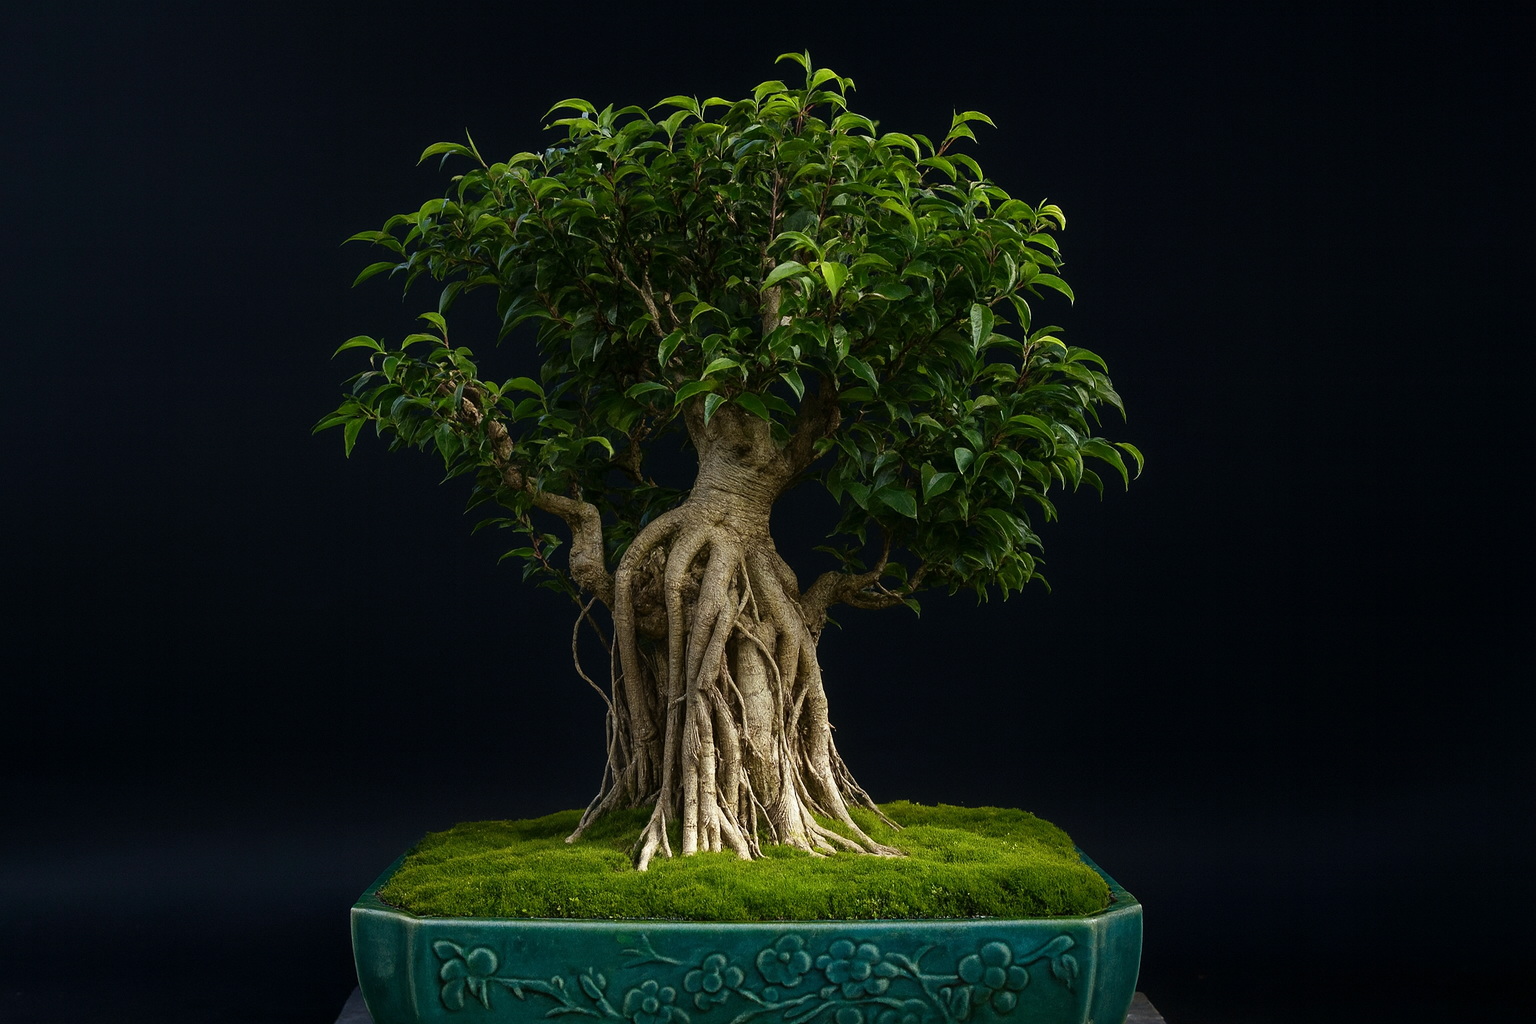
\includegraphics[width=1.0\columnwidth]{2025_11/res/wired_frankenficus},\centerline{\emph{The `Frankenficus' proves make\--do\--and\--mend works wonders.}}]
\end{window}
\clearpage

\noindent
Winters can drop to \mbox{$\--30^\circ$C}, summers rise to \mbox{$30^\circ$C}, and protection is essential.
Nigel now maintains a greenhouse, a polyhouse, a warm plant room, and a cool one---each allowing him to cultivate a remarkable variety of species.
Even so, pests and climate extremes remain perennial tests.

Some species---especially those from deserts or tropical climates---are exceptionally sensitive.
They can thrive under perfect conditions yet decline rapidly after the smallest mistake.
Nigel accepts this as part of the pursuit.

Patience is key to his long\--term motivation.
Rather than chasing show trees, he finds joy in annual progress, however subtle.
``\textit{If you're only after impressive show trees, you may never enjoy the day\--to\--day work. For me, bonsai is about the process of development---the pursuit of the unobtainable goal of perfection.}''

Older trees sometimes require difficult decisions.
Resetting a mature root system or making a drastic cut can be nerve\--wracking, but occasionally necessary.
Nigel recalls reducing the roots of a twenty\--seven\--year\--old ficus by ninety percent---a terrifying moment, but one that ultimately improved the tree.

Looking ahead, Nigel hopes simply to keep learning.
As his trees gain maturity, some may eventually enter shows.
He also dreams of expanding his outdoor garden area with more benches, though this may mean reducing the number of trees he keeps.
Quality over quantity becomes more important with time.

\medskip
\topic{Closing Thoughts}
\noindent
Asked what advice he would give beginners, Nigel responds without hesitation: ``\textit{Study trees in nature. Learn what makes an oak look different from a maple. Don't rush. Trees grown slowly with care always look better than those pushed too quickly.}''

He emphasises the importance of continual learning and open\--mindedness.
Listen to everyone, he suggests, then decide what resonates with your own goals.
Above all, enjoy the time you have---both with the trees and in life.

When asked for one word to describe bonsai, he replies simply: \textbf{Dedication}.

To him, the community is an essential part of that dedication.
A solitary backyard hobby can transform into a vibrant, lifelong social connection: ``\textit{A group of like\--minded friends is a good thing. Bonsai has survived 2\,000 years, and I'm happy to be part of that history.}''

\begin{center}
    $\cdots$
\end{center}

\noindent
We thank Nigel for sharing his time, his story, and his steady, generous approach to both bonsai and life.
His trees, and his videos, continue to inspire across generations and continents---inviting us all into the Bonsai Zone.
\closearticle

\vfill
\end{multicols}

\begin{center}
\begin{minipage}[b]{.48\textwidth}
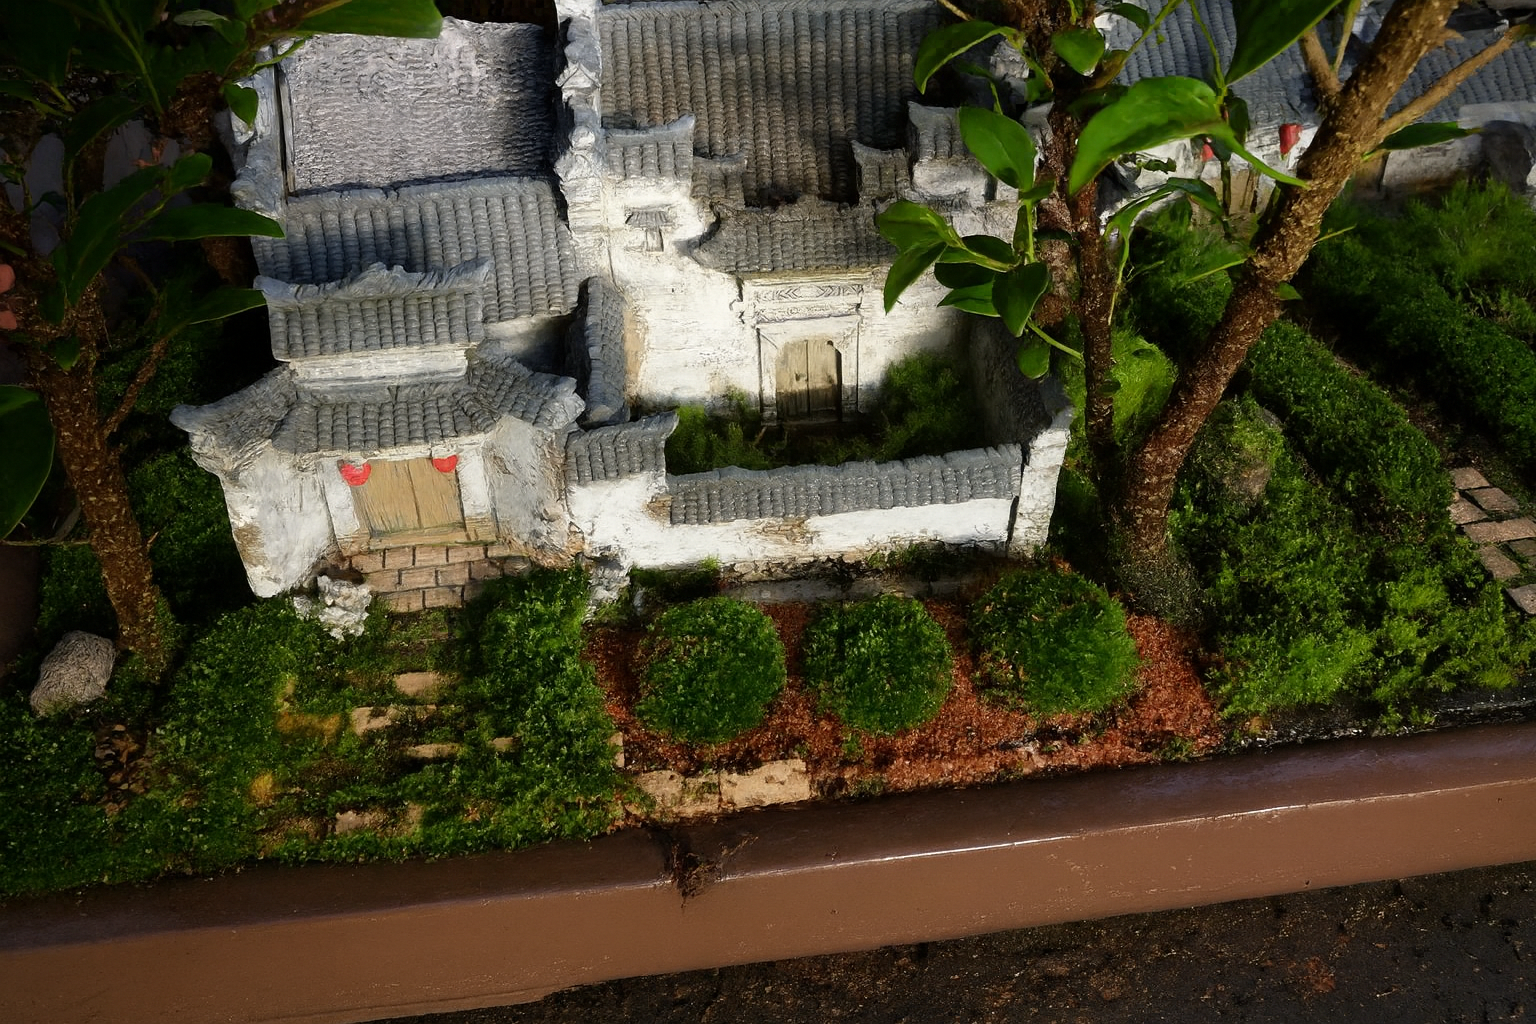
\includegraphics[angle=0,origin=c,width=1.0\textwidth]{2025_11/res/wired_penjing}
\end{minipage}\quad
\begin{minipage}[b]{.48\textwidth}
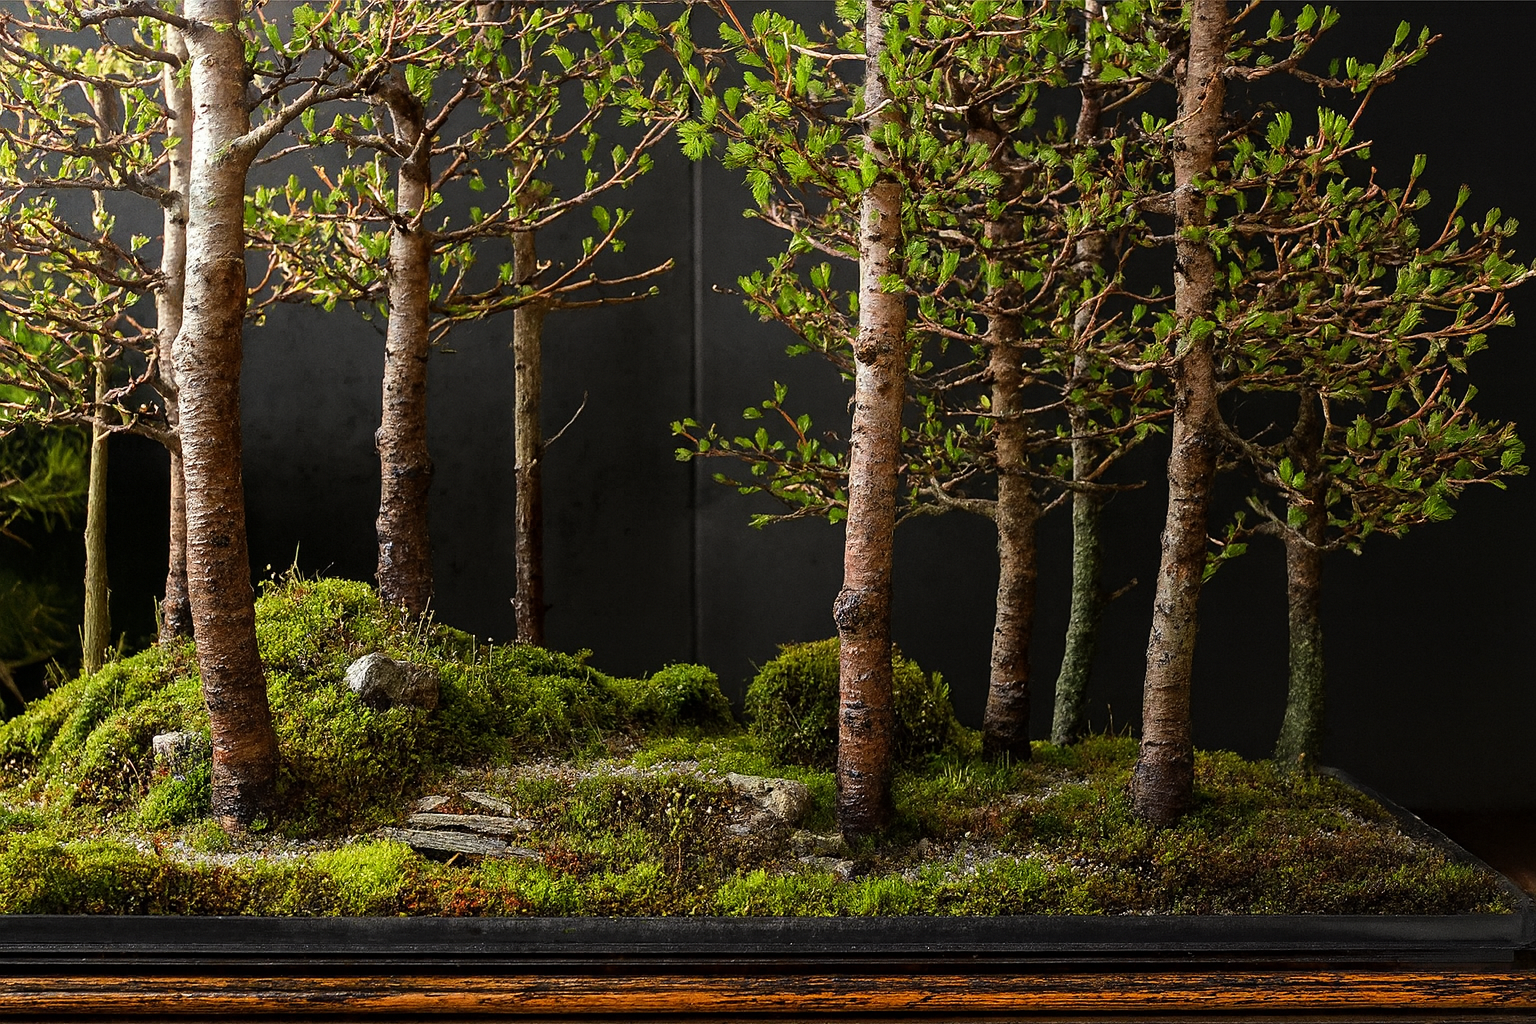
\includegraphics[angle=0,origin=c,width=1.0\textwidth]{2025_11/res/wired_forest}
\end{minipage}
\medskip

\begin{minipage}[b]{.48\textwidth}
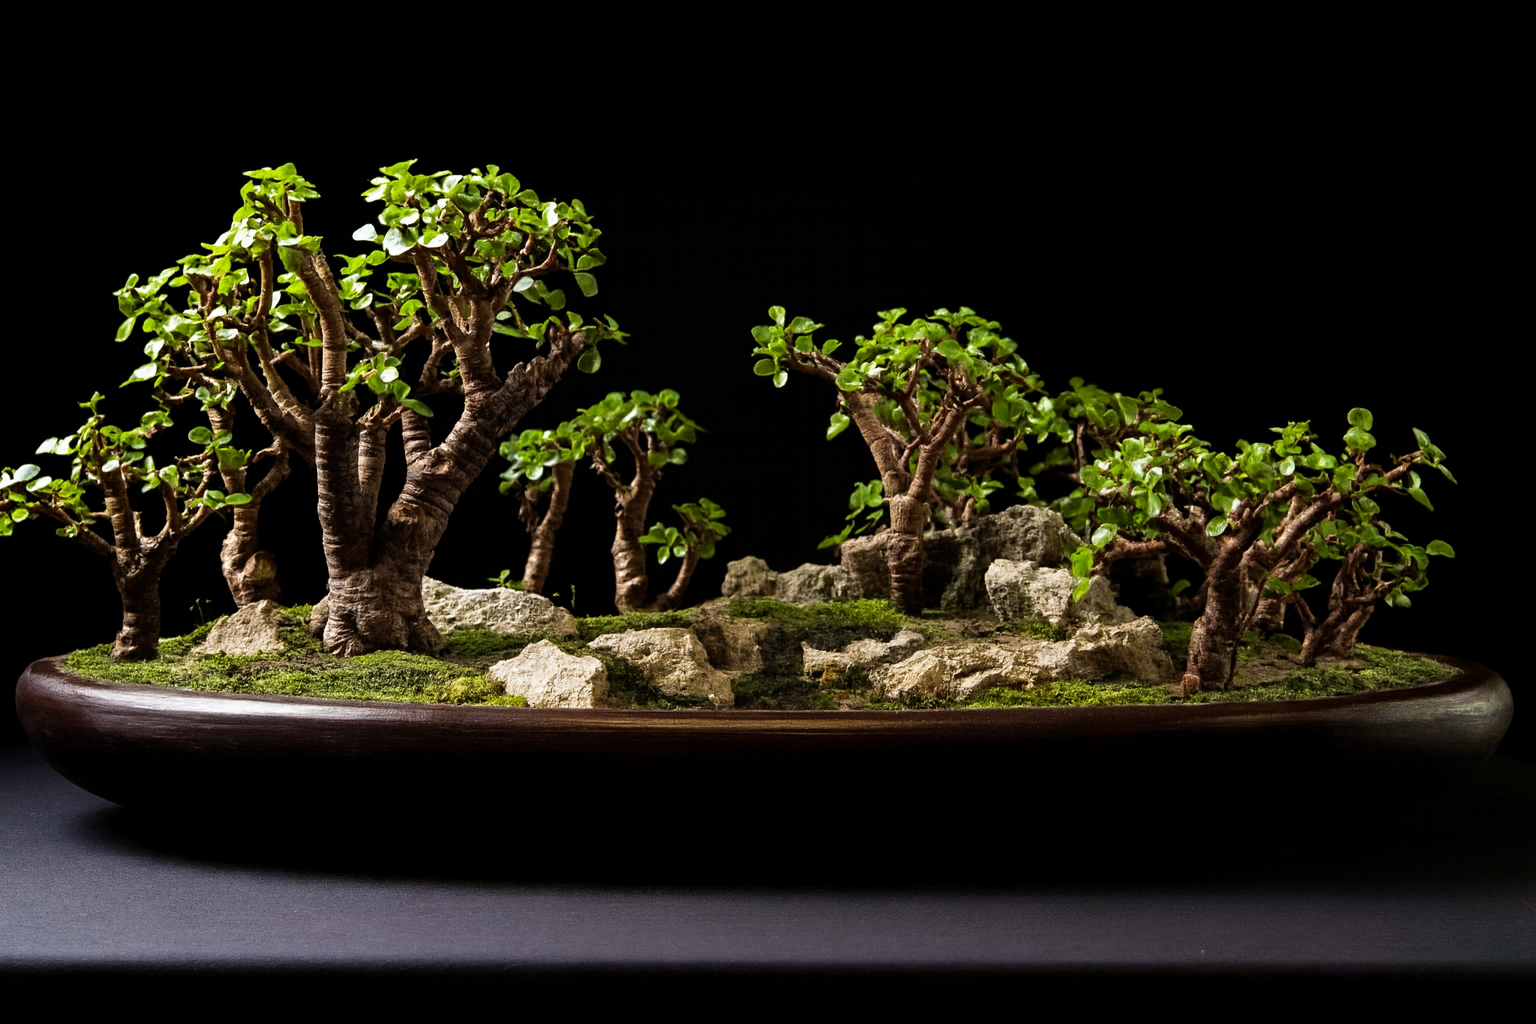
\includegraphics[angle=0,origin=c,width=1.0\textwidth]{2025_11/res/wired_kabu}
\end{minipage}\quad
\begin{minipage}[b]{.48\textwidth}
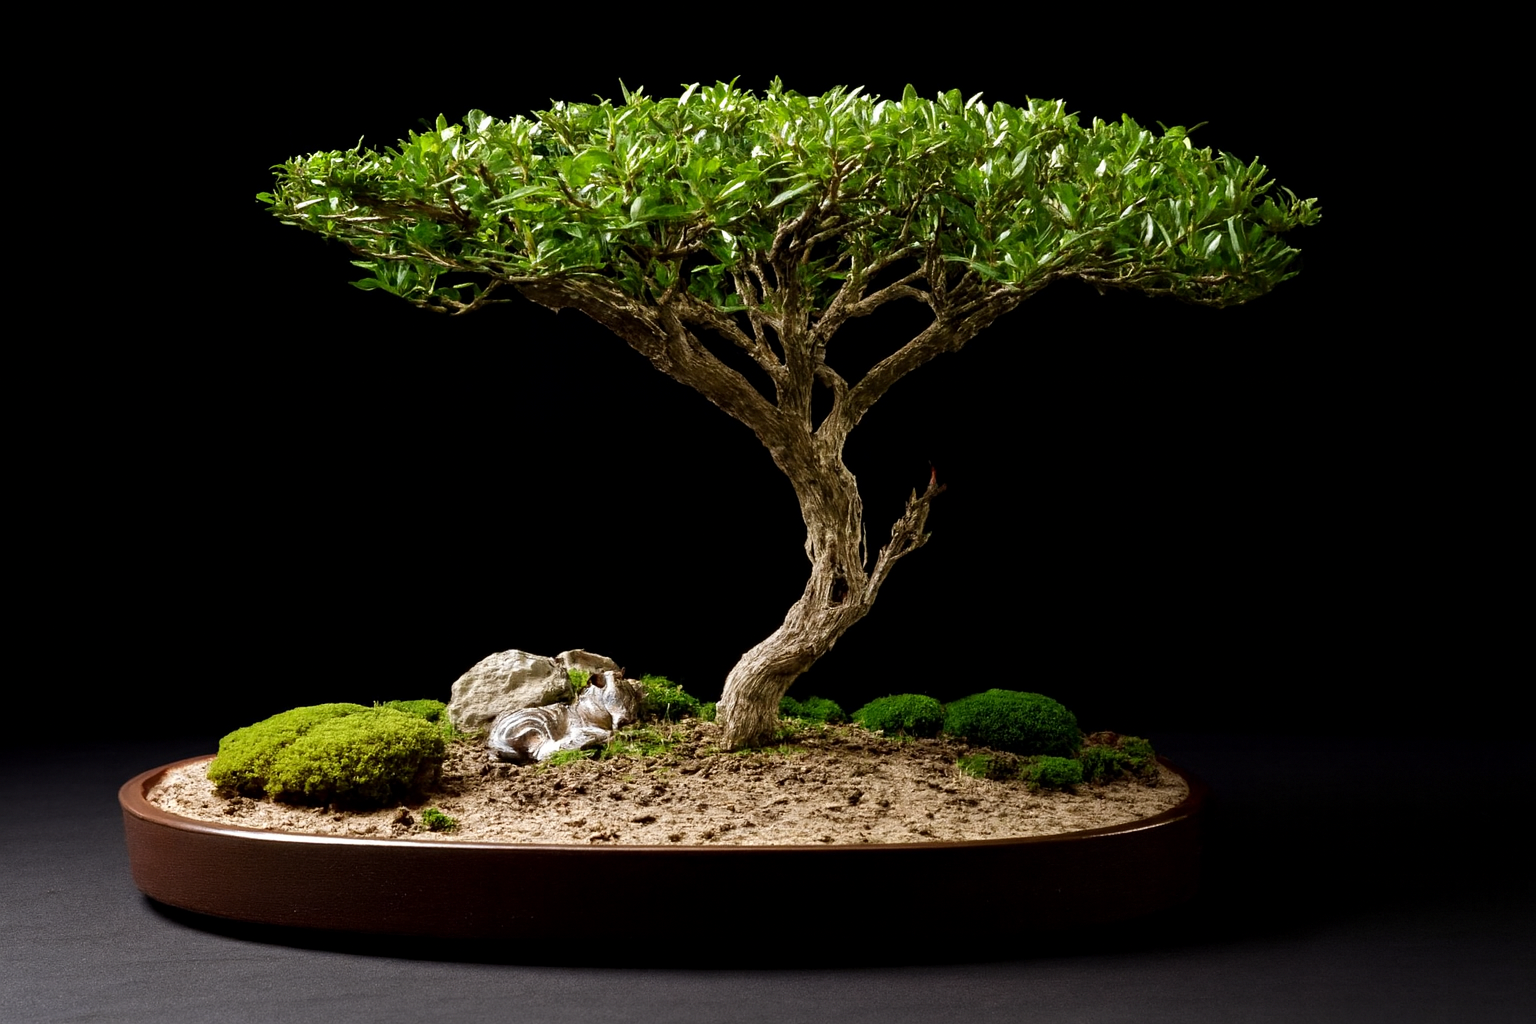
\includegraphics[angle=0,origin=c,width=1.0\textwidth]{2025_11/res/wired_pierneef}
\end{minipage}
\end{center}
\centerline{\emph{Breaking the mold: Nigel Saunders' naturalistic and unusual styles have been celebrated in many bonsai shows.}}

\begin{multicols}{2}
\clearpage
